\textbf{Agenda}

Pada chapter ini kita akan membahas mengenai bahasa C dan Qt Cretor 
seperi berikut ini

\minitoc

\section{Pengenalan Bahasa C++}\label{pengenalan-bahasa-cpp}



Bahasa C merupakan bahasa pemrograman tingkat menengah. Pada tahun 1972
bahasa C pertama kali dirancang oleh \index{Dennis M Ritchie}
\href{https://id.wikipedia.org/wiki/Dennis_Ritchie}{Dennis M Ritchie}\footnote{https://id.wikipedia.org/wiki/Dennis\_Ritchie}{Dennis M Ritchie} di
Bell aboratories. Kemudian tahun 1978 Dennis dan\index{Brian W. Kernighan} 
\href{https://id.wikipedia.org/wiki/Brian_Kernighan}{Brian W. Kernighan}\footnote{https://id.wikipedia.org/wiki/Brian\_Kernighan}{Brian W. Kernighan}
mempublikasikan bahasa C melalui \index{The C
	Programming Language}
\href{https://id.wikipedia.org/wiki/The_C_Programming_Language}{The C
Programming Language}\footnote{https://id.wikipedia.org/wiki/The\_C\_Programming\_Language} sehingga bahasa C dikenal banyak orang.
Selanjutnya pada tahun 1989, akhirnya bahasa C distandardisasi \index{ANSI}
\href{https://id.wikipedia.org/wiki/ANSI_C}{ANSI}\footnote{https://id.wikipedia.org/wiki/ANSI\_C} (American National
Standard Institute) sehingga bahasa C menjadi bahasa pemrograman standar
hingga saat ini dan bisa dibuat kompilernya pada beberapa platform yang
berbeda-beda.

Bahasa C dikatakan sebagai bahasa pemrograman terstruktur, fungsional
karena strukturnya menggunakan fungsi-fungsi sebagai program-program
bagian (subroutine/ module). Fungsifungsi selain fungsi utama disebut
subroutine/ module dan ditulis setelah fungsi utama (main) atau
diletakkan pada file pustaka (library). Jika fungsi-fungsi diletakkan
pada file pustaka dan akan dipakai disuatu program, maka nama file
header-nya harus dilibatkan dalam program menggunakan preprocessor
directive \texttt{\#include}.

Kemudian bahasa C dikembangkan oleh Bjarne Stroustrup at Bell Labs
menjadi bahasa C++. Pada bulan Oktober 1985 munculah buku \emph{The C++
Programming Language} yang membahas tentang bahasa pemrograman itu
langsung dari penciptanya sendiri. Bahasa C++ mengalami dua tahap
evolusi.

\begin{itemize}

\item
  Pertama, dirilis oleh
  \href{https://id.wikipedia.org/wiki/Bell_Laboratories}{AT\&T
  Laboratories}\footnote{Bell Laboratories (juga dikenal dengan nama Bell Labs dan sebelumnya dengan nama AT\&T Bell Laboratories dan Bell Telephone Laboratories) adalah bagian dari organisasi riset dan pengembangan dari Alcatel-Lucent dan sebelumnya dari United States Bell System.}, dinamakan
  \href{https://en.wikipedia.org/wiki/Cfront}{cfront}\footnote{https://en.wikipedia.org/wiki/Cfront}. C++ versi ini
  hanya berupa kompiler yang menterjemahkan bahasa C++ menjadi bahasa C
  untuk dieksekusi
\item
  Kedua, \href{https://en.wikipedia.org/wiki/Borland}{Borland
  International Inc}\footnote{Borland Software Corporation adalah sebuah perusahaan perangkat lunak komputer yang berkantor pusat di Austin, Texas. Perusahaan ini didirikan pada tahun 1983 oleh Niels Jensen, Ole Henriksen, Mogens Glad dan Philippe Kahn.}. mengembangkan kompiler C++ menjadi sebuah kompiler
  yang mampu mengubah C++ langsung menjadi bahasa mesin (assembly).
  Tahun1990, C++ mulai diarahkan ke pengembangan
  \href{https://id.wikipedia.org/wiki/Pemrograman_berorientasi_objek}{Pemrograman
  Berorientasi Obyek}\footnote{OOP (Object Oriented Programming) adalah suatu metode pemrograman yang berorientasi kepada objek. Tujuan dari OOP diciptakan adalah untuk mempermudah pengembangan program dengan cara mengikuti model yang telah ada di kehidupan sehari-hari.}.
\end{itemize}

Beberapa keunggulan C++ dibandingkan dengan bahasa C adalah sebagai
berikut.

\begin{description}

\item[Object-oriented programming]
Bahasa pemrograman ini sangat mendukung pemrograman berorientasi obyek
yang melihat permasalahan secara obyek dan bukan prosedural.
\item[Portability]
Kita dapat mengkompilasi C++ kode yang sama di hampir semua jenis
komputer dan sistem operasi tanpa membuat perubahan apapun. C++ adalah
bahasa pemrograman yang paling sering digunakan di dunia.
\item[Brevity]
Karena bahasa C++ merupakan bahasa tingkat tinggi, maka bahasa yang
ditulis dengan bahasa C++ termasuk ringkas dan pendek dibandingkan
bahasa-bahasa sejamannya pada waktu itu.Bahasa C++ termasuk bahasa
pemrograman tua yang sudah mendukung berbagai macam kata kunci yang
mampu menyingkat proses penulisan kode program.
\item[Modular programming\footnote{pemrograman modular adalah mengelompokkan fungsi-fungsi utama kedalam sebuah modul, dimana tiap-tiap modul memiliki datanya masing-masing dan mampu mengolah datanya sendiri. Modul-modul ini yang akan digunakan dalam program.}]
Tubuh program pada bahasa C++ dapat terdiri dari beberapa file source
code yang disusun secara terpisah dan kemudian dihubungkan secara
bersama-sama. Kemampuan ini jelas menghemat waktu karena tidak perlu
mengkompilasi ulang aplikasi yang lengkap ketika membuat satu perubahan,
tetapi hanya file yang berisi perubahan itu saja. Selain itu,
karakteristik ini memungkinkan kita untuk menghubungkan kode C++ dengan
kode yang dibuat oleh bahasa lain, seperti bahasa Assembly dan C dan
dapat digunakan kembali (reuseable).
\item[C Compatibility]
C++ sangat backward compatible dengan bahasa C, sehingga aplikasi / kode
program yang ditulis dengan bahasa C dapat digabungkan dengan bahasa C++
dengan sangat mudah, bahkan hampir tidak perlu mengubah kodenya.
\item[Speed]
Kode yang dihasilkan dari kompilasi C++ sangat efisien, karena C++
mendukung prinsip dualitas bahwa dia mendukung bahasa tingkat tinggi dan
bahasa tingkat rendah sehingga dapat mengurangi ukuran hasil kompiliasi
dari bahasa itu.
\end{description}

\section{Pengantar Qt Creator}\label{pengantar-qt-creator}

Qt Creator merupakan cross-platform C++ integrated development
environment yang merupakan bagian dari Qt SDK \index{Qt SDK}. Qt Creator mempunyai
debugger dalam bentuk visual dan layout GUI \index{GUI} serta tempat perancangan
form. Teks editornya mempunyai fasilitas syntax highlighting dan
autocompletion. Qt Creator menggunakan compiler C++ dari kumpulan
compiler \index{GNU}GNU pada \index{Linux}Linux dan \index{FreeBSD}FreeBSD. Pada Windows \index{Windows} Qt Creator dapat
menggunakan MinGW\footnote{minGW adalah salah satu aplikasi yng
  digunakan untuk mengkompile bahasa C agar dapat dipahami oleh bahasa
  mesin (asembler) pada komputer. Aplikasi ini dapat di unduh secara
  gratis.} atau
\href{https://id.wikipedia.org/wiki/Microsoft_Visual_Studio_Express}{MSVC}\footnote{sebuah perangkat lunak lengkap (suite) yang dapat digunakan untuk melakukan pengembangan aplikasi, baik itu aplikasi bisnis, aplikasi personal, ataupun komponen aplikasinya, dalam bentuk aplikasi console, aplikasi Windows, ataupun aplikasi Web. Visual Studio mencakup kompiler, SDK, Integrated Development Environment (IDE), dan dokumentasi (umumnya berupa MSDN Library). Kompiler yang dimasukkan ke dalam paket Visual Studio antara lain Visual C++, Visual C\#, Visual Basic, Visual Basic .NET, Visual InterDev, Visual J++, Visual J\#, Visual FoxPro, dan Visual SourceSafe.}
yang sudah build-in di dalam install.

Project Qt Creator menggunakan format cross platform project (.pro)
untuk mengizinkan tim developer untuk share project yang mempunyai
platform-platform yang berbeda-beda dan menggunakan common tool untuk
implementasi dan debugging program. Sebuah project dapat meliputi:

file-file yang digroup secara bersama-sama, langkah-langkah build
program, form-form dan file-file resource, dan pengaturan untuk
menjalankan aplikasi.

Projek dapat dibuat secara manual atau diimport dari file projek yang
sudah ada. Jika projeknya dibuat secara manual, maka sebuah file-file
akan digenerate oleh Qt Creator, tergantung dari tipe file yang
dimiliki. Seperti Jika filenya adalah sebuah GUI application, maka Qt
Creator men-generate sebuah file kosong yang berektensikan \texttt{.ui}
yang akan imodifikasikan melalui Qt Designer\index{Qt Designer}. Qt Creator diinterrasikan
dengan sistem cross-platform untuk mem-build secara automatis: qmaka\index{qmake} dan CMake
\index{CMake}. Projek yang tidak menggunakan qmake atau CMake dapat
diimport-kan, dan Qt Creator dapat meng-ignore sistem build.

\begin{figure}[htbp]
\centering 
\includegraphics[width=0.6\textwidth]{images/capture1-1.png}
\caption{Projek pada Qt Creator}
\end{figure}\label{projek-pada-qt-creator}

Editor Qt Creator mempunyai sebuah code editor yang telah terintegrasi
dengan Qt Designer untuk mendesain dan membangun aplikasi GUI dari \index{Qt
	widgets}Qt
widgets. Karena Qt Creator adalah sebuah Integrated Development
Enviroment (IDE), maka Qt Creator memisahkan antara text editor untuk
build dan editor untuk menjalankan (run) aplikasi-aplikasi. Qt Creator
bukan hanya bisa membaca text file biasa, akan tetapi juga bisa membaca
file C++ dan bahasa QML \index{QML}.

Keunggulan Code Editor Qt Creator

\begin{itemize}

\item
  Dapat menulis code dengan format yang benar.
\item
  Mengantisipasikan apa yang akan programer tulis dan code yang komplit.
\item
  Menampilkan baris-baris yang error dan pesan-pesan warning.
\item
  Memandu programer secara semantik untuk menulis classes, functions,
  dan symbols.
\item
  Menyediakan fasilitas bantuan context-sensitive pada classes,
  functions, dan symbols.
\item
  Me-rename symbol-symbol dengan langkah intelligent, sehingga
  simbol-simbol yang lain dengan nama yang sama tidak ter-rename.
\item
  Menampilkan lokasi function, class yang dideklarasikan atau yang
  dipanggil
\end{itemize}

\begin{figure}[htbp]
\centering
\includegraphics[width=0.8\textwidth]{images/capture1-2.png}
\label{code-editor}
\caption{ Code Editor}
\end{figure}

\subsection{UI Designer}\label{ui-designer}

Qt Creator menyajikan dua buah editor visual: \index{Qt Designer}Qt Designer  dan \index{Qt Quick	Designer}Qt Quick
Designer. Qt Designer merupakan sebuah tool untuk mendesain dan
membangun aplikasi GUI dari \index{Qt widgets}Qt widgets. Widgets dan forms yang dibentuk
dengan Qt Designer terintegrasi dengan code program, Qt signals dan
mekanisme slots, sehingga kita dengan mudah memberikan nilai-nilai dan
properti-properti pada pada elemen-elemen grafik. Semua
properti-properti yang diatur pada Qt Designer dapat diubah secara
dinamik melalui/di dalam code.

Qt Quick Designer digunakan untuk membangun secara mudah animasi-animasi
dengan menggunakan sebuah bahasa pemograman yang dikenal dengan
\href{https://en.wikipedia.org/wiki/QML}{Qt Meta-Object Language (QML)}\footnote{https://en.wikipedia.org/wiki/QML}.
Dalam QML, sebuah user interface dispesifikasikan sebagai sebuah pohon
(tree) dari objects dengan properti-properti. Kamu menggunaan teks
editor visual untuk menciptakan items, screens, dan aplikasi, serta
mendefinisikan perubahan action-acton pada komponennya. Dapat digunakan
Qt atau JavaScript untuk mengimplementasikan logik aplikasi.

\begin{figure}[htbp]
\centering
\includegraphics[width=0.8\textwidth]{images/capture1-3.png}
\caption{Gambar UI Designers}
\end{figure}\label{gambar-ui-designers}

\subsection{Bahasa yang di dukung}\label{bahasa-yang-di-dukung}

Anda dapat menggunakan code editor menulis code dalam Qt C++ atau bahasa
pemograman QML, javascript bahkan HTML5. Syntax highlighting juga
disajikan untuk banyak bahasa pemograman yang lain.

\subsection{Platform}\label{platform}

Qt Creator men-support untuk membangun dan menjalankan aplikasi-aplikasi
Qt untuk desktop environments (Seperti Windows, Linux, FreeBSD dan Mac
OS) Selain itu juga bisa dijalankan pada mobile devices (seperti
Android, windows 8 dan iOS). Ketika sebuah aplikasi dibangun untuk
mobile device yang bisa mengkoneksi ke Personal Computer (PC), maka Qt
Creator men-generate sebuah package instalasi, menginstall package
tersebut pada device, dan meneksekusikannya.

\subsection{Tools}\label{tools}

Qt Creator diintegrasikan dengan kumpulan tool-tool yang bermanfaat dan
membantu, seperti version control systems dan Qt Simulator. Qt Creator
menggunakan command line client version control system untuk mengakses
repositories (\href{https://git-scm.com/}{Git}\footnote{Git adalah tools yang berfungsi sebagai Version Control System (VCS) dan kalau diartikan ke bahasa kita artinya sebuah sistem pelacak perubahan pada file. Git sendiri dibuat oleh orang yang menciptakan Kernel Linux, yup... tidak salah lagi dia adalah yang mulia Linus Torvalds.},
\href{https://subversion.apache.org/}{subversion}\footnote{Subversion (SVN) adalah salah satu version control system popular yang ada. SVN mula-mula diciptakan sebagai pengganti CVS, software yang popular sebelumnya namun memiliki banyak kelemahan.},
\href{https://www.perforce.com}{Perfoce}\footnote{https://www.perforce.com},
\href{www.nongnu.org/cvs/}{CVS}\footnote{Computer vision syndrome (CVS) adalah suatu keadaan yang terjadi karena terlalu lama memfokuskan mata pada layar komputer. Umumnya penderita akan mengeluhkan nyeri kepala, pusing, penglihatan kabur, nyeri leher, mata merah, penglihatan ganda, sulit memfokuskan mata, bahkan kelelahan.},
\href{https://www.mercurial-scm.org}{Mercurial}\footnote{Mercurial adalah salah satu software revision control yang dikembangkan dengan menggunakan Python, dan tersedia untuk beberapa platform seperti Linux, Windows dan MacOS.  Tidak seperti software revision control lain yang sudah lama dipakai seperti CVS dan SVN, Mercurial menggunakan distributed revision control.  Dengan demikian, tidak ada satu server pusat yang berisi repository source-code (koleksi kode program).  Setiap orang dapat mengambil source code dari sebuah repository, kemudian membuat repository-nya sendiri.}).

\subsection{Debuggers}\label{debuggers}

Qt Creator tidak mempunyai debugger. Qt Creator mempunyai plugin
debugger yang bekerja sebagai interface antara Qt Creator core dan
external native debuggers

Debuggers adalah:

\begin{itemize}

\item
  GNU Symbolic Debugger (gdb)
\item
  Microsoft Console Debugger (CDB)
\item
  internal Java Script debugger
\end{itemize}

Dapat menghubungkan mobile devices dengan PC dan memproses debug yang
berjalan pada devices.

\section{Mengenal macam - macam Teknologi User Interface (UI)
pada
QT}\label{mengenal-macam-macam-teknologi-user-interface-ui-pada-qt}

Interaksi antara pengguna dengan logic software dinamakan User Interface
disingkat dengan UI. UI ini berwujud bisa sebuah window, bisa tombol,
bisa sebuah textarea dan lain sebagainya. Inilah komponen User
Interface. Sebagai seorang programmer (pembuat program aplikasi),
terlebih programmer yang menggunakan Qt, maka anda akan disediakan
beragam UI yang bisa anda pilih sesuai kebutuhan. Ada QtWitget, QtQuick
dan QtWebKit. Ketiganya dapat anda pilih sesuai kebutuhan sebagai UI
progam anda. Ingin tahu bedanya? Mari kita simak.

Sama seperti Visual Studio yang menyediakan beragam Amazing User
Interface tingkat tinggi sampai pengguna bingung memilihnya, Qt
menyediakan tiga UI yang dapat kita gunakan. Anda pun bisa menggabungkan
ketiganya. :)

Qt Creator, sebuah Editor Qt adalah contoh dari perpaduan multiple
teknologi UI ini. Coba amati Qt Creator yang selalu anda gunakan
tersebut.

Qt Creator menggunakan teknologi QtWidget sebagai User Interface pada
menu dan kotak dialog nya. Coba perhatikan kembali Welcome Screen dari
Qt Creator, lihat, tampilannya berbeda bukan, bahkan button nya sangat
berbeda dan tidak biasa, ini karena UI untuk Welcome Screen menggunakan
teknologi QtQuick. Lalu dimana letak penggunaan QtWebkit?

Yup, perhatikan Help Documentation nya, wow, ini seperti halaman web
yang menyatu dengan softwarenya bukan? Ya, teknologi QtWebKit digunakan
dalam pembangunan Help Documentation ini.

\subsection{Teknologi User Interface
QtQuick}\label{teknologi-user-interface-qtquick}

QtQuick merupakan salah satu Teknologi UI dari Qt yang menggunakan QML
dan JavaScript sebagai penyusun UI nya.Mirip seperti XAML yang
dikembangkan Microsoft , QML merupakan teknologi binding dari Qt yang
memfasilitasi pengguna dengan visual canvas dan rendering engine nya.
Teknologi UI ini sangat cocok sekali untuk Hardware Acceleration seperti
OpenGL pada VGA driver kita.

Jangan salah, bila anda menggunakan QtQuick versi 2, maka memang butuh
OpenGL yang disuport oleh VGA anda. OpenGL sekarang begitu terkenal,
banyak games - games yang mulai menargetkan OpenGL karena begitu
flexibel dan mudah. Tapi sayangnya, OpenGL ini tidak terdapat pada VGA
driver bawaan OS.

Jadi jangan heran, saat anda install ulang komputer (bahkan Windows 8.1
sekalipun) anda akan menemukan bahwa tidak ada OpenGL pada VGA driver
anda. Cara terbaik adalah periksa Motherboard anda dan cari driver VGA
yang sesuai dengan Motherboard anda. Biasanya gratis.

Animation, Transition, Visual Effect, Shader Effect dan lain -- lain
merupakan fasilitas yang dapat anda kembangkan saat menggunakan QtQuick
sebagai User Interface (UI) aplikasi anda.

\subsection{Teknologi User Interface
QtWidget}\label{teknologi-user-interface-qtwidget}

QtWidget merupakan tradisional User Interface element yang biasanya
terdapat dalam dekstop environment. Bila anda pengguna linux, maka UI
ini merupakan bagian dari KDE. Tapi jangan salah, QtWidget sangat
dinamis untuk Windows dan Mac OS. Sehingga bila anda menggunakan
QtWidget sebagai UI anda maka tampilannya mirip sekali dengan UI pada OS
anda.

Bila anda pengguna Windows 8.1 seperti saya dengan Amazing Flat
Designnya, maka QtWidget ini menyesuaikan dengan UI OS.

Semua standar komponen untuk aplikasi seperti button, textarea, menu dan
lain -- lain terdapat pada QtWidget ini. Sehingga sangat cocok sekali
untuk anda yang gemar membuat aplikasi tradisional standar.

Bila kita membuat aplikasi dengan QtWidget, maka saat memulai project,
akan muncul pemilihan Base Class, ada tiga yaitu Class QWidget, Class
QMainWindow, dan Class Qdialog.

Perbedaan dari ketiga Base Class di atas adalah berikut ini:

\begin{itemize}
\item
  \texttt{*QWidget} merupakan base class untuk semua GUI element pada
  QtWidget User Interface. Coba lah explorasi dan bedakan ketiganya :)
\item
  \texttt{*QDialog} merupakan sebuah window yang biasanya digunakan
  untuk mengejutkan pengguna, seperti saat window dialog muncul ketika
  pengguna harus memasukan input dengan benar atau hal -- hal yang lain,
  tampilan dari Qdialog tidak berbeda dengan Qwidget, anda bisa
  menggunakan salah satu.
\item
  \texttt{*QMainWindow}, nah, ini adalah sebuah class yang sangat unik,
  karena menggunakan feature \emph{built in} yang sangat populer seperti
  status bar, toolbar, dan menu bar. Cobalah membuat applikasi QtWidget
  dengan QmainWindow sebagai base class nya, pasti secara otomatis akan
  ditampilan menubar , toolbar, dan statusbar.
\end{itemize}

\subsection{Teknologi User Interface
QtWebkit}\label{teknologi-user-interface-qtwebkit}

Tahukah anda bahwa web programing adalah kegiatan yang paling berkembang
di dunia saat ini? Tahukah anda bahwa web koding seperti html, css, js
sangat populer dan mudah digunakan dan mulai merambah ke teknologi
desktop seperti Html5\footnote{HTML5 adalah sebuah bahasa markah untuk menstrukturkan dan menampilkan isi dari World Wide Web, sebuah teknologi inti dari Internet. HTML5 adalah revisi kelima dari HTML dan hingga bulan Juni 2011 masih dalam pengembangan.} dan CSS3\footnote{CSS3 adalah Cascading Style Sheet versi ke 3, yaitu pengatur dan pengendali tampilan sebuah halaman blog/ web. CSS3 melakukan penataan terhadap komponen HTML maupun XHTML pada halaman web sehingga menghasilkan tampilan yang ramah dimata atau retina friendly.}?

Lalu kenapa tidak digunakan dalam pemrograman desktop? Ya, dengan
menggunakan User Interface QtWebkit\footnote{WebKit adalah sebuah Mesin Layout yang didesain agar browser dapat merender halaman web. Webkit adalah komponen dasar dari penjelajah web Apple Safari dan Google Chrome. Pada bulan juli 2012, berdasarkan StatCounter - webkit mendapatkan lebih dari 40 \% kue di pasar penjelajah web. Webkit menjadi dasar utama pada browser default di iOS, Android, Tablet Blackberry, dan sistem operasi webOS. Webkit menyediakan sekumpulan kelas untuk menampilkan isi pada jendela dan menerapkannya pada fitur penjelajah web, misalnya : mengikuti tautan ketika di-klik oleh pengguna, mengatur daftar kembali-maju, dan rekaman halaman yang baru saja dikunjungi.} ini anda bisa membuat sebuah desktop\footnote{Komputer meja (bahasa Inggris: desktop computer atau cukup desktop saja) adalah komputer pribadi yang ditujukan untuk penggunaan secara umum di satu lokasi yang berlawanan dengan komputer jinjing atau komputer portabel. Periferal-periferal komputer meja seperti tampilan komputer, CPU, dan papan ketik terpisah satu sama lain dan relatif berukuran besar (juga berlawanan dengan periferal pada komputer jinjing yang terintegrasi dan berukuran kecil). Komputer jenis ini dirancang untuk diletakkan dan digunakan di atas meja di rumah atau kantor. Komputer meja merupakan komputer yang paling terjangkau dan paling umum digunakan.}
application dengan menggunakan koding web. Unik bukan?

Teknologi QtWebkit menampilkan web content melalui QML, sedangkan C++
API digunakan untuk interaksi dengan web content tersebut.

Perlu diperhatikan bersama bahwa pemilihan teknologi adalah biasa, so,
tetaplah berkreasi, berikut kita kutipkan beberapa perbandingan antar
tiga teknologi UI dari Qt Help Documentation.

\section{ Install Qt Creator}\label{install-qt-creator}

Pada tutorial ini kita akan menginstall Qt pada ubuntu 14.04 atau
Windows 8 dengan menggunakan versi terbaru dari Qt Creator yang dapat di
unduh di \href{http://www.qt.io/download}{halaman}\footnote{https://www.qt.io/download-open-source/\#section-2} Qt cCreator.

\begin{figure}[htbp]
\centering
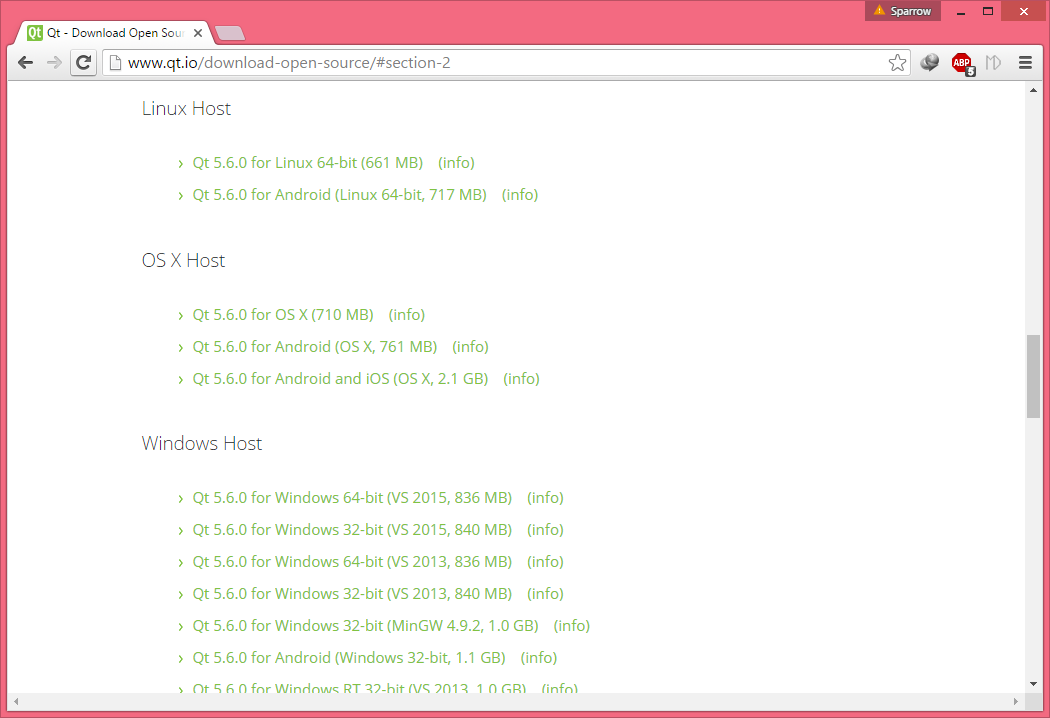
\includegraphics[width=0.8\textwidth]{images/qt-downloads.png}
\label{halaman-web-download-qt}
\caption{Halaman web Downlaod Qt Creator}
\end{figure}

\subsection{Install Qt Creator di Ubuntu
14.04}\label{install-qt-creator-di-ubuntu-14.04}

\paragraph{1. Download}\label{download}

Kunjungi website Qt untuk mendowload Qt Crator sesui dengan versi sisem
operasi yang di gunakan baik itu 64-bit atau 32 bit. atau juga dapat di
download dengan menggunakan command line di linux dengan mengetikan.

Contoh:

\begin{lstlisting}[language=sh, numbers=none]
wget http://download.qt.io/official_releases/online_installers/qt-unified-linux-x86-online.run
\end{lstlisting}

jika menggunakan sistem operasi beberbasis 64 bit

\begin{lstlisting}[language=sh, numbers=none]
wget http://download.qt.io/official_releases/qt/5.6/5.6.0/qt-opensource-linux-x64-5.6.0.run
\end{lstlisting}

\paragraph{2. Install}\label{install}

Atur permisi, jalankan installer dan ikuti perintah berikut ini untuk
mnginstall Qt Creator secara lengkap.

\begin{lstlisting}[language=sh, numbers=none]
chmod +x qt-opensource-linux-x64-5.6.0.run
./qt-opensource-linux-x64-5.6.0.run
\end{lstlisting}

\paragraph{3. Install g++}\label{install-gpp}

Buka terminal untuk menginstal g++:

\begin{lstlisting}[language=sh, numbers=none]
sudo apt-get install build-essential
\end{lstlisting}

\paragraph{4. K0nfigurasi Kompiler}\label{k0nfigurasi-kompiler}

Buka Qt Creator klik tool \textgreater{} Options. Klik build \& run dan
pilih tab Kit. Konfigurasikan kompiler jka belum terdeteksi secara
otomatis.

\paragraph{5. Install Pustaka OpenGL}\label{install-pustaka-opengl}

Jalankan Perintah berikut ini mengintall Pustaka OpenGL:

\begin{lstlisting}[language=sh, numbers=none]
sudo apt-get install mesa-common-dev
\end{lstlisting}

\subsection{Install Qt di Windows}\label{install-qt-di-windows}

Anda dapat mendownlod Qt creator di halaman websitenya seperti gambar \ref{halaman-web-download-qt} dan memlilih versi
dari Aplikasi yang Anda butuhkan baik 64 bit atau 32 bit. Sesuikan
dengan sistem operasi yang Anda miliki.

\paragraph{Langkah 1}
  Jika Anda telah mendownlaod Qt creator maka
  \textit{qt-opensource-windows-x86-mingw492-5.5.0.exe}. Disini penulis
  menggunakan versi 32 bit jika sistem oeprasi Anda 64 bit maka
  gunakanlah 64 bit walaupun dapat menggunakan versi 32 bit.
 
\begin{center}
	 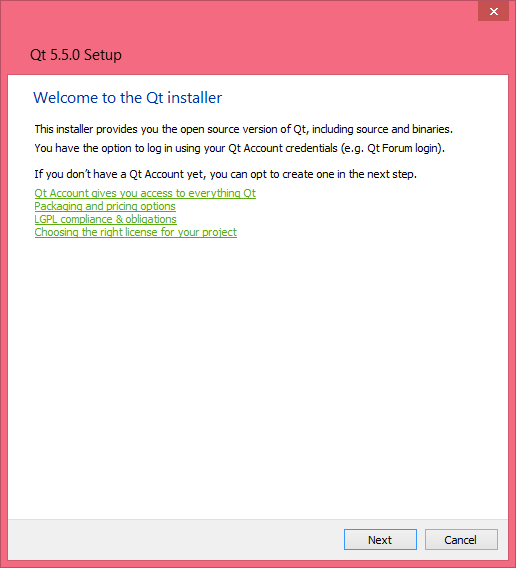
\includegraphics[width=0.4\textwidth]{images/install-qt-1.png}
\end{center}
 



\paragraph{Langkah 2}
  Pilih \textbf{Next} dan akan muncul halaman Qt Acount jika anda tidak
  ingin mendatarkan diri dapat di lewati dengan memilih \textbf{skip}.

\begin{center}
	 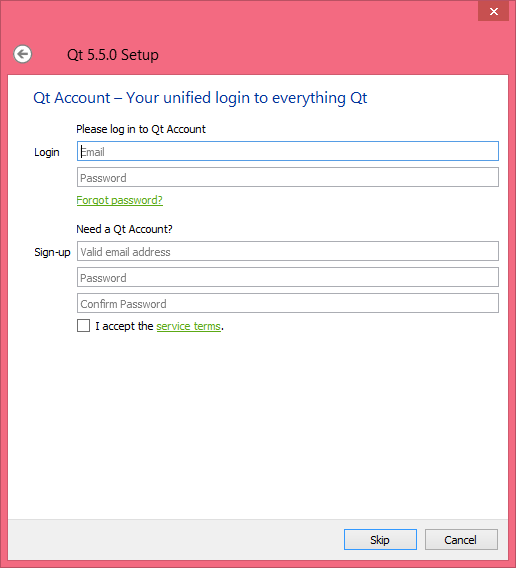
\includegraphics[width=0.4\textwidth]{images/install-qt-2.png}
\end{center}
 


  
\paragraph{Langkah 3}
  Masuk ke halaman Setup terus \textbf{next} saja.

  
\begin{center}
	 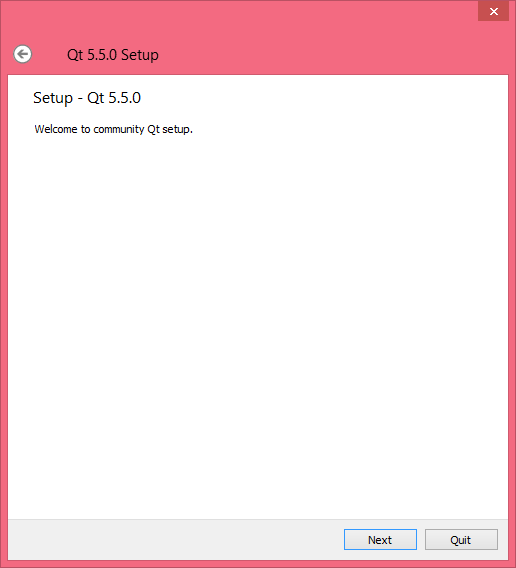
\includegraphics[width=0.4\textwidth]{images/install-qt-3.png}
\end{center}
 


  
\paragraph{Langkah 4}
  Installer akan menginstall aplikasi sampai selesai apabila telah
  selesai maka klik finish untuk mengakhiri proses pemasangan aplikasi.


  


\begin{center}

	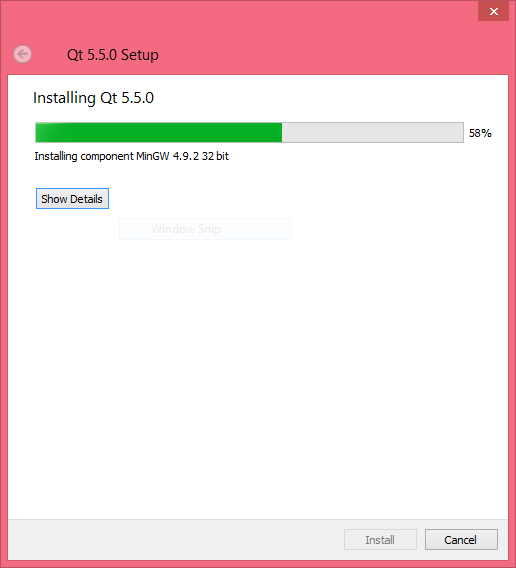
\includegraphics[width=0.4\textwidth]{images/install-qt-4.png}
\end{center}

\section{Program Console Pertama dengan Qt
Creator}\label{program-console-pertama-dengan-qt-creator}



  Untuk mencoba membuat aplikasi dengan Qt Creator maka kita perlu
  dengan membuat menu file \textgreater{} new Project dan pilih project
  aplication \textgreater{} Qt console aplication

  \begin{center}

  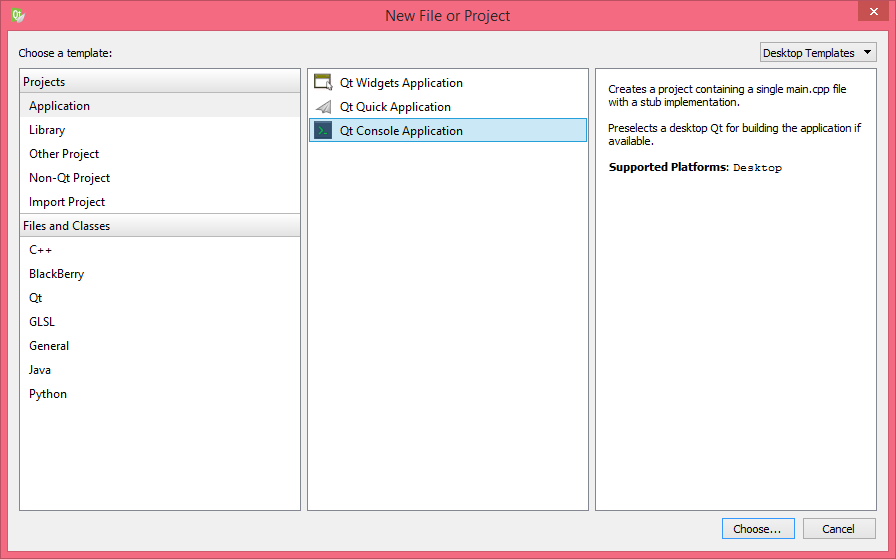
\includegraphics[width=0.8\textwidth]{images/qt-console-aplication.png}

  \end{center}

  kemudian beri nama dengan Program yang akan kita buat dan direktori
  tempat aplikasi yang kita buat.

  \begin{center}

  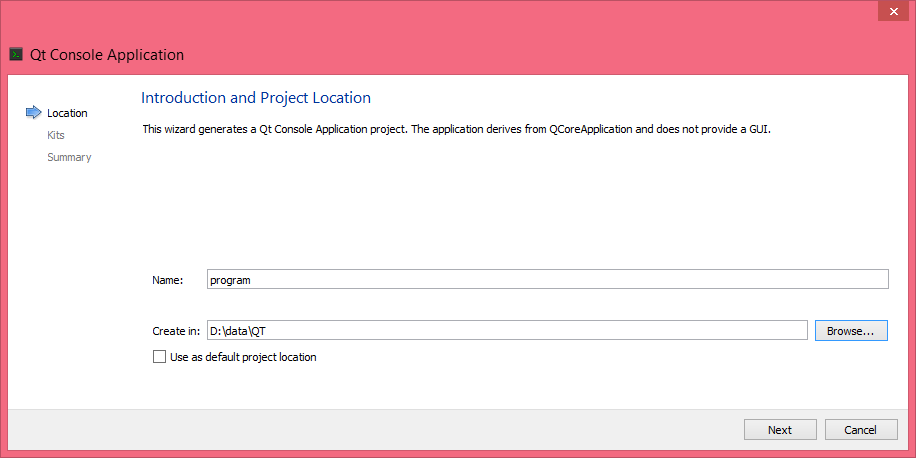
\includegraphics[width=0.8\textwidth]{images/qt-console-aplication-2.png}

  \end{center}

  Klik Next, kemudian pilih compiler yang akan kita gunakan. Disini
  penulis menggunakan MinGW sebagai compilernya.


\begin{quotation}
	\textbf{Tips}
	
	Simulator 	 atau compiler yang lengkap teridir dari
	
	\begin{itemize}
		
		\item
		Qt Simulator MingGW 4.4
		\item
		Qt Simulator VS 2008, 2010, 2011, 2012 2013, 2014
		\item
		Android SDK dan NDK
	\end{itemize}
\end{quotation}




\begin{center}

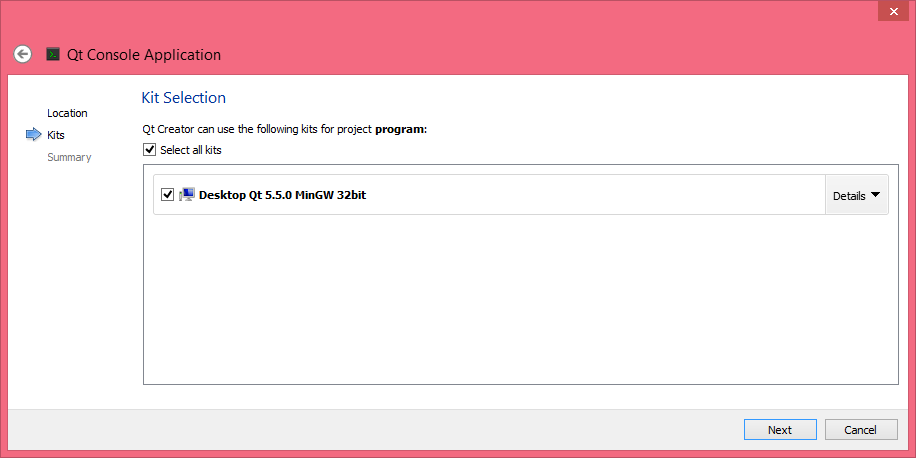
\includegraphics[width=0.8\textwidth]{images/qt-console-aplication-3.png}

\end{center}

\begin{enumerate}

\setcounter{enumi}{3}

\item
  Kemudian pilih jenis sub version yang akan kita gunakan, jika Anda
  tidak mengunakan sub version maka pilih none pada add to subversion.
\end{enumerate}

\begin{figure}[htbp]
\centering
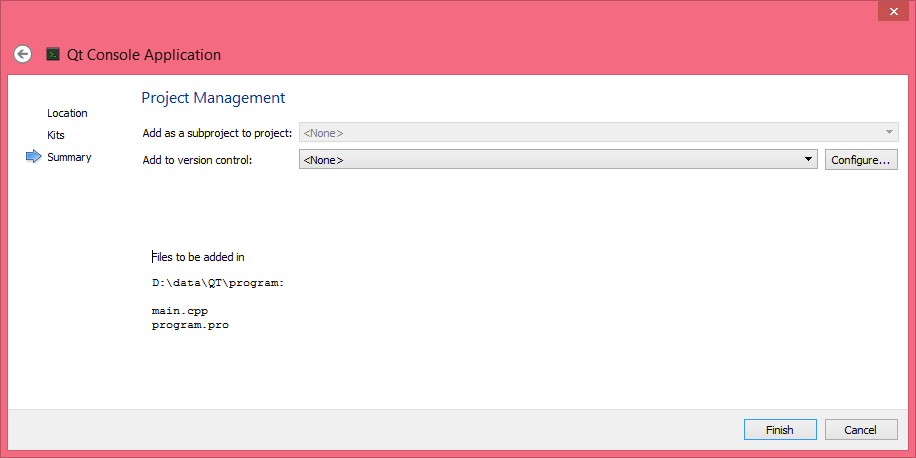
\includegraphics[width=0.8\textwidth]{images/qt-console-aplication-4.png}
\caption{Langkah 1 Setup Qt Creator }
\end{figure}

\begin{enumerate}

\setcounter{enumi}{4}

\item
  Apabila di lakukan dengan benar maka akan muncul Qt Editor sebagai
  berikut ini.
\end{enumerate}

\begin{center}

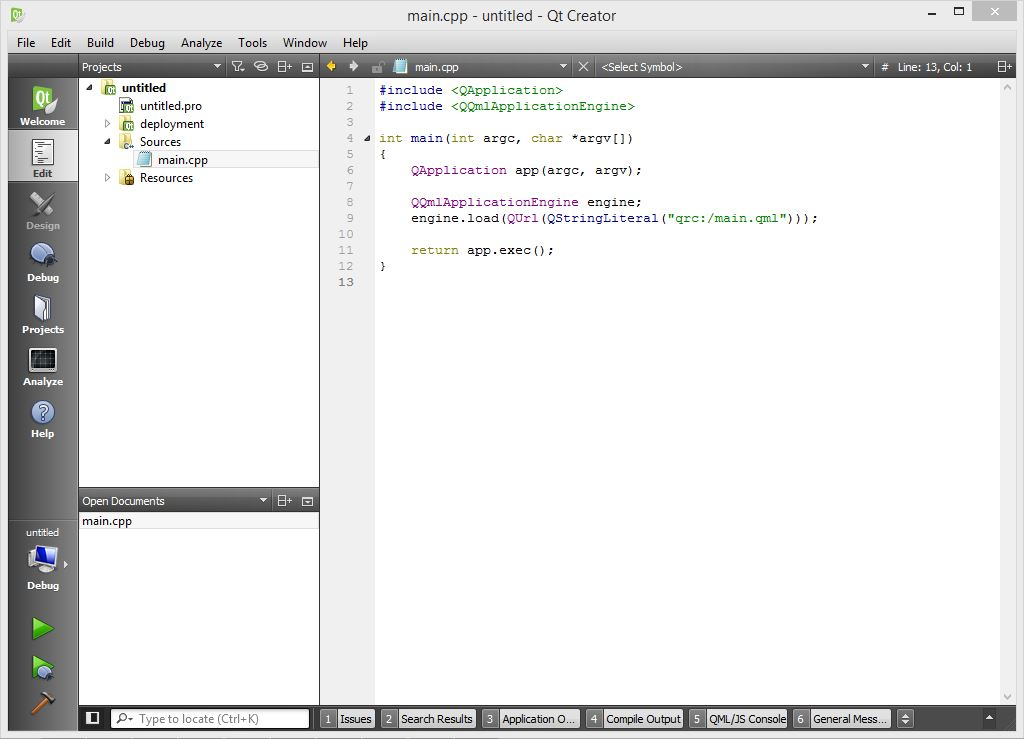
\includegraphics[width=0.8\textwidth]{images/qt-creator.jpg}

\end{center}

\section{Struktur Program C++}\label{struktur-program-cpp}

Program Bahasa C/C++ tidak mengenal aturan penulisan di kolom/baris
tertentu, jadi bisa dimulai dari kolom/baris manapun. Namun demikian,
untuk mempermudah pembacaan program dan untukkeperluan dokumentasi,
sebaiknya penulisan program di bahasa C/C++ diatur sedemikian rupa
sehingga mudah dan enak dibaca. Berikut adalah struktur dasar program
yang dibuat dengan bahasa C++:

\begin{lstlisting}[language=c++, caption=Struktur Program C++]
#include <header>  
using namespace std;    
int main(int argc, char *argv[])
{  
deklarasi variabel;   
deklarasi konstanta;  
perintah perintah;  
//komentar  
return 0;  
}  
\end{lstlisting}

\textbf{Penjelasan :}

\paragraph{ 1. \#include <header>}

\texttt{\#include} adalah salah satu pengarah preprocessor directive
yang tersedia pada C++. Preprocessor selalu dijalankan terlebih dahulu
pada saat proses kompilasi terjadi. Bentuk umumnya:

\begin{lstlisting}[language=c++, numbers=none]
# include <nama_file>
\end{lstlisting}

Bagian tersebut tidak diakhiri dengan tanda semicolon, karena bentuk
tersebut bukanlah suatu bentuk pernyataan, tetapi merupakan preprocessor
directive. Baris tersebut menginstruksikan kepada kompiler untuk
menyisipkan file lain dalam hal ini file yang berakhiran .h (file
header) yaitu file yang berisi C++ standard library. Pada C++ ekstensi
.h tidak dituliskan.

Beberap contoh pengikutsertaan berkas adalah:

\begin{itemize}

\item
  \texttt{\#include\ \textless{}iostream\textgreater{}} : diperlukan
  pada program yang melibatkan objek \texttt{cout} dan \texttt{cin}
\item
  \texttt{\#include\ \textless{}conio\textgreater{}}: diperlukan bila
  melibatkan \texttt{clrscr()}, yaitu perintah untuk membersihkan layar
  dan fungsi \texttt{getch()} untuk menerima sembarang input keyboard
  dari user.
\item
  \texttt{\#include\ \textless{}iomanip\textgreater{}} : diperlukan bila
  melibatkan \texttt{setw()} yang bermanfaat untuk mengatur lebar dari
  suatu tampilan data.
\item
  \texttt{\#include\ \textless{}math\textgreater{}} : diperlukan pada
  program yang menggunakan operasi \texttt{sqrt()} yang bermanfaat untuk
  operasi matematika kuadrat.
\end{itemize}

\paragraph{2. using namespace std;}\label{using-namespace-std}

Semua elemen standard C++ library dinyatakan dalam apa yang disebut
namespace, namespace tersebut bernama std. Jadi artinya untuk mengakses
semua fungsionalitas std kita menuliskan bahwa kita menggunakan
namespace std.

\paragraph{3. int main ()}\label{int-main}

Program C++ terdiri dari satu atau lebih fungsi, dan di antara salah
satunya harus ada fungsi main dan hanya boleh ada satu main pada tiap
program C++. Setiap program C++ akan dan pasti akan memulai eksekusi
programnya pada fungsi main ini, meskipun main bukan fungsi yang pertama
ditulis di program. Melihat bentuk seperti itu dapat kita ambil
kesimpulan bahwa batang tubuh program utama berada didalam fungsi
main(). Berarti dalam setiap pembuatan program utama, maka dapat
dipastikan seorangpemrogram menggunakan minimal sebuah fungsi.

Tanda \{ dan pada akhir program terdapat tanda \}. Tanda \{ harus ada
pada setiap awal dari sebuah fungsi dan tentu saja harus diakhiri dengan
tanda \}. Tanda ini digunakan untuk menunjukkan cakupan(scope) dari
sebuah fungsi,dimana untukmenunjukkan fungsi ini dimulai danberakhir.

\paragraph{4. Komentar}\label{komentar}

Komentar tidak pernah dicompile oleh compiler. Dalam C++ terdapat 2
jenis komentar, yaitu:

\begin{lstlisting}[language=c++, numbers=none]

  /* Komentar anda diletakkan
   di dalam ini bisa mengapit
    lebih dari satu  baris */

  // Komentar anda diletakkan disini
  // ( hanya bisa sebaris )
\end{lstlisting}

Programmer sering sekali memasukkan komentar di dalam code agar program
lebih mudah dibaca. Komentar juga membantu orang lain untuk membaca dan
mengerti isi dari code. Komentar tidak menyebabkan komputer melakukan
suatu instruksi ketika program dijalankan.

\paragraph{5. Tanda Semicolon (;)}\label{tanda-semicolon}

Tanda semicolon `` \texttt{;} '' digunakan untuk mengakhiri sebuah
pernyataan. Setiap pernyataan harus diakhiri dengan sebuah tanda
semicolon.

\paragraph{9. return 0}\label{return-0}

Pernyataan return menyebabkan fungsi utama untuk menyelesaikan
kegiatannya lalu mengembalikanhasil dari fungsi utama. Kode kembalian
biasanya angka 0 atau 1. Jika angka yang dikembalikan 0 berartiprogram
berakhir dengan tidak ada error, sedangkan jika 1 maka program berakhir
dengan error.

\subsubsection{Contoh Structur program C++}

Untuk lebih jelasnya silahkan coba ketik program berikut pada project
baru.

\begin{lstlisting}[language=c++, caption= Contoh struktur program C++]
#include <QtCore/QCoreApplication>  
#include <iostream>  
using namespace std;  
int main (int argc, char *argv [])  
{  
QCoreApplication a (argc, argv);  
cout<<"Hello World"<<endl;  
cout<<"Selamat Belajar C/C++ ";  
cout<<"enter my World";  
return a.exec ();  
}
\end{lstlisting}

Kemudian jalankan dengan menekan tombol Run (CTRL + R)

\begin{lcverbatim}
Hello world
Selamat belajar C/C++ enter my world
\end{lcverbatim}


Tampilan Hello World diakhiri dengan tanda enter baru kemudian
dilanjutkan dengan tulisan berikutnya yaitu Selamat Belajar C/C++ enter
my World. Artinya perintah \texttt{endl} merupakan perintah untuk
memberi tanda enter. Sedangkan untuk tulisan Selamat Belajar C/C++ dan
tulisan enter my World yang pada source code terpisah dengan perintah
\texttt{cout}, pada tampilan hasil program tetap sama dan tidak ada
enter diantaranya. Hal ini karena tidak ada perintah untuk menampilkan
enter diantara kedua kalimat tersebut. Penulisan pada kode tidak akan
mempengaruhi hasil output program.
